\documentclass[../ai_in_finance]{subfiles}
\usepackage[margin=1in]{geometry}
\usepackage{tikz}
\usetikzlibrary{positioning}
\usepackage{amsmath}
\usepackage{amssymb}
\usepackage{booktabs}
\usepackage{floatrow}
\usepackage{draftwatermark}

\SetWatermarkText{Wulin.Suo@Queensu.ca}
\SetWatermarkScale{1.4}
\SetWatermarkColor{gray!35}
\SetWatermarkAngle{45}

\usepackage{makeidx}
\makeindex

\begin{document}

\chapter{Case Studies and Capstone Projects}

\section{Introduction}

Every dataset used so far in this book, Cascade Home\index{Cascade Home \& Garden} \& Garden's satellite-derived car counts, Meridian Fabrication\index{Meridian Fabrication Inc.}'s financial statements, the ten-transaction fraud-scoring sample, was constructed for a single purpose: to make one method's mechanics checkable by hand, uncluttered by the messiness real data always carries. That was the right choice for teaching each method in isolation, but it leaves an honest gap this closing chapter exists to fill: a real financial dataset, of the kind a working data scientist actually downloads from a public repository such as the UCI Machine Learning Repository or Kaggle, arrives with undocumented category codes, an imbalanced target, correlated and redundant features, and no guarantee that the model that wins on one metric also wins on every other metric that matters. This chapter works a single such dataset end to end, using nothing but tools this book has already built, feature engineering (Chapter 6), a model bake-off spanning linear and tree-based methods (Chapters 6 and 15), calibration\index{calibration} (a genuinely new topic, motivated directly by Chapter 9's own caveat that a credit score is only meaningful if its underlying probability is accurate), real explainability tooling (Chapter 16's SHAP\index{SHAP} and permutation-importance methods, now run with the actual \texttt{shap} library rather than by hand), a cost-sensitive threshold choice (extending Chapter 13's alert economics), and a real fairness audit (extending Chapter 16's synthetic two-group example with genuine data), before closing with governance considerations and a set of further capstone project ideas for the reader to pursue independently.

Two further, more advanced analyses push past what a first pass through this pipeline would typically include: a systematic hyperparameter search quantifying exactly how much is actually gained by tuning a model beyond a single, reasonable configuration, and an intersectional fairness cut that splits the test population two ways at once and uncovers a clear four-fifths-rule violation that this chapter's own single-attribute fairness audit, run first, entirely missed.

The dataset is the \emph{Default of Credit Card Clients} dataset (Yeh and Lien, 2009), 30,000 Taiwanese credit card accounts with 23 raw features and a binary label, default on payment the following month, hosted on the UCI Machine Learning Repository and also widely distributed on Kaggle under the same name, exactly the kind of source this chapter's title points to. Unlike every other dataset in this book, it was not built to illustrate anything in particular, and working through it surfaces problems no fictional dataset would: undocumented category codes that must be cleaned before any model can be fit, a real 22.1\% default rate rather than a convenient round number, and, as this chapter's fairness audit shows directly, results close enough to a regulatory threshold that the same model could plausibly land on either side of it depending on which quarter's data a bank happened to audit.

This chapter's structure mirrors the order a working data scientist actually follows on a new dataset, and is worth previewing before working through the details. It begins where any real project begins, inspecting the raw data closely enough to find its undocumented quirks (Section~\ref{sec:capstone-data}) and engineering features from raw monthly statements rather than starting from an already-clean feature table (Section~\ref{sec:capstone-features}). It then compares several model families on identical, held-out data (Section~\ref{sec:capstone-bakeoff}), checks whether the winning model's probabilities can actually be trusted at face value (Section~\ref{sec:capstone-calibration}), explains that model's behavior using real software rather than hand computation (Section~\ref{sec:capstone-explain}), converts model output into an actual lending decision using an explicit cost assumption (Section~\ref{sec:capstone-threshold}), and audits that decision for fairness, first along one dimension and then, in Section~\ref{sec:capstone-advanced}, along two dimensions at once (Section~\ref{sec:capstone-fairness}). A closing discussion of what deploying this pipeline in production would actually require (Section~\ref{sec:capstone-governance}) distills that same pipeline into an explicit, reusable template (Section~\ref{sec:capstone-template}), before a set of further capstone projects to apply it to (Section~\ref{sec:capstone-projects}) end the chapter, and the book, on the same note the introduction to Chapter 1 opened it: these tools are only as trustworthy as the discipline applied in using them.

\section{The Capstone Dataset and Its Imperfections}\index{Capstone Dataset and Its Imperfections}
\label{sec:capstone-data}

The raw dataset records, for each of 30,000 accounts, a credit limit (\texttt{LIMIT\_BAL}), demographic fields (\texttt{SEX}, \texttt{EDUCATION}, \texttt{MARRIAGE}, \texttt{AGE}), six months of repayment status codes (\texttt{PAY\_1} through \texttt{PAY\_6}, where $-1$ indicates payment made duly and a positive integer indicates the number of months a payment is overdue), six months of billed amounts (\texttt{BILL\_AMT1}--\texttt{BILL\_AMT6}), six months of amounts actually paid (\texttt{PAY\_AMT1}--\texttt{PAY\_AMT6}), and the target, default on the following month's payment. Loading the data immediately surfaces the first real-world imperfection this chapter's fictional datasets never had: the data dictionary documents \texttt{EDUCATION} as taking values 1 (graduate school), 2 (university), 3 (high school), or 4 (other), yet the actual column also contains 14 rows coded 0, 280 rows coded 5, and 51 rows coded 6, none of which the documentation defines. \texttt{MARRIAGE} shows the same pattern: documented as 1 (married), 2 (single), or 3 (other), the column also contains 54 rows coded 0. Neither anomaly is disclosed anywhere in the dataset's documentation, and a modeler who does not notice them will silently feed a machine learning model category codes with no defined meaning. Following the standard practice for this well-studied dataset, both sets of undocumented codes are folded into their respective ``other'' categories (0, 5, and 6 into \texttt{EDUCATION}'s existing category 4; 0 into \texttt{MARRIAGE}'s existing category 3) before any modeling begins, a cleaning step with no equivalent anywhere else in this book precisely because every other dataset was built clean by construction.

Table~\ref{tab:capstone_summary} summarizes four representative raw fields before any cleaning or feature engineering, and is itself worth inspecting closely rather than skimming past, exactly the habit Chapter 6 recommended before fitting any model to any dataset.

\begin{table}[htbp]
\centering
\caption{Summary statistics for four raw fields (before cleaning)}
\label{tab:capstone_summary}
\begin{tabular}{lrrrrr}
\toprule
Field & Mean & Std.\ dev. & Min & Median & Max \\
\midrule
\texttt{LIMIT\_BAL} (NT\$) & 167{,}484 & 129{,}748 & 10{,}000 & 140{,}000 & 1{,}000{,}000 \\
\texttt{AGE} (years) & 35.5 & 9.2 & 21 & 34 & 79 \\
\texttt{BILL\_AMT1} (NT\$) & 51{,}223 & 73{,}636 & $-165{,}580$ & 22{,}382 & 964{,}511 \\
\texttt{PAY\_AMT1} (NT\$) & 5{,}664 & 16{,}563 & 0 & 2{,}100 & 873{,}552 \\
\bottomrule
\end{tabular}
\end{table}

\texttt{BILL\_AMT1}'s negative minimum is a third genuine data quirk beyond the two category-code anomalies above, not documented anywhere in the dataset's description: a negative billed amount means the account was in credit, having overpaid the previous month, rather than owing anything at all, a legitimate state for a revolving credit account but one that a modeler unfamiliar with the data might mistake for a data-entry error and drop or clip without justification. \texttt{PAY\_AMT1}'s heavy right skew, a median of just NT\$2,100 against a mean of NT\$5,664 and a maximum of NT\$873,552, is exactly the kind of distribution Section~\ref{sec:capstone-features}'s engineered ratio features are designed to normalize before they reach a linear model, though the tree-based models in Section~\ref{sec:capstone-bakeoff} are considerably less sensitive to this kind of skew than logistic regression\index{logistic regression} is, since a tree splits on a feature's rank order rather than its raw scale.

Two further properties of the raw data are worth noting before any model is fit. First, the 22.1\% default rate is considerably higher than a typical, real-world consumer credit-card portfolio, which more commonly runs in the low single digits, a reminder that a published research dataset's class balance reflects however it happened to be sampled or the period it happened to be drawn from (this data covers a six-month window in 2005, shortly before a Taiwanese consumer-credit crisis), not necessarily the class balance any other institution's own portfolio will show; a model built on this chapter's data should not be assumed to transfer its absolute predicted probabilities to a materially different portfolio without recalibration, even if its ranking of relatively risky against relatively safe accounts transfers reasonably well. Second, several of the raw features are highly correlated with each other by construction, the six \texttt{BILL\_AMT} columns track a single account's revolving balance from one month to the next and therefore move together closely, which matters directly for Section~\ref{sec:capstone-explain}'s explanation exercise: an importance or attribution score assigned to any one of several mutually correlated features is, to some extent, arbitrary, since a model can typically substitute one for another with little effect on its predictions, an issue Chapter 6 raised in the abstract when discussing multicollinearity in linear regression and that carries over, in a different technical form, to tree-based models and their explanations alike.

\section{From Raw Fields to Model-Ready Features}\index{From Raw Fields to Model-Ready Features}
\label{sec:capstone-features}

Chapter 6 introduced feature engineering in the abstract; this section performs it on genuinely raw fields for the first time. Four engineered features summarize the six months of repayment and billing history into a form a model can use more directly than six separate monthly columns each: \texttt{max\_delinquency}, the worst (maximum) repayment-status code across all six months, a single number capturing whether an account was ever seriously overdue even if its most recent month looks clean; \texttt{avg\_utilization}, the average, across the six months, of billed amount divided by credit limit, a standard credit-risk signal Chapter 9 introduced conceptually but never computed from raw statement data; \texttt{total\_bill} and \texttt{total\_paid}, the six-month sums of billed and paid amounts; and \texttt{pay\_to\_bill\_ratio}, the ratio of the two, capturing how much of what an account owed it actually paid back over the window, clipped at 5 to bound the influence of a small number of accounts with an unusually large payment relative to a near-zero bill. These, together with the 23 raw fields, give 28 features in total.

The 30,000 accounts are split 80/20 into a training set of 24,000 and a held-out test set of 6,000, stratified by the default label so that both sets preserve the same 22.1\% default rate, using a fixed random seed so the split (and every result in this chapter) is exactly reproducible from the companion notebook. Every model comparison, calibration check, explanation, threshold choice, and fairness audit in the rest of this chapter is computed on this same held-out test set, never on the data any model was fit to, the discipline Chapter 6 introduced as essential to detecting overfitting\index{overfitting} and that matters more, not less, once a real dataset's quirks make it easy to convince oneself a model has learned something it has only memorized.

One further discipline is worth naming explicitly because a real dataset makes it easy to violate by accident: every one of this section's engineered features, \texttt{max\_delinquency} included, is computed from information available at the time each account's repayment history was recorded, not from anything that depends on knowing whether the account actually defaulted. This sounds obvious, but Chapter 15's point-in-time discipline for alternative data applies here in a more subtle form: a feature engineered carelessly from a dataset that also contains the outcome column, for instance a rolling average that accidentally incorporates a future month's billing data, can leak information about the label into the features and produce a model that looks excellent on a held-out test set drawn from the same leaking dataset, yet fails immediately once deployed on genuinely new applicants for whom that same leakage is not available. This dataset's structure happens to make such leakage easy to avoid, since every raw field precedes the single target month by construction, but the discipline of checking for it explicitly, not merely assuming a clean-looking dataset has none, is exactly the habit a reader should carry into Section~\ref{sec:capstone-projects}'s further projects, several of which (the Lending Club dataset in particular) are considerably easier to leak by accident than this one.

\begin{figure}[htbp]
\centering
\begin{lrbox}{\bookmeasuredbox}
    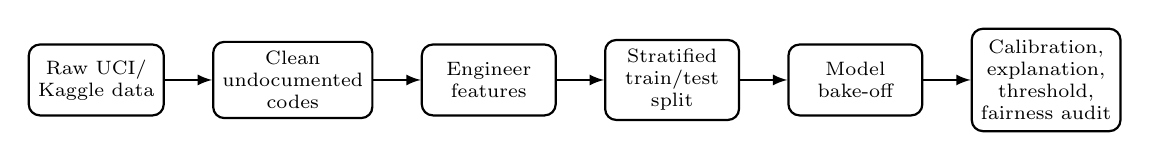
\begin{tikzpicture}[>=latex,thick,node distance=0.6cm]
        \node[draw,rounded corners,minimum width=1.7cm,minimum height=0.9cm,align=center,font=\scriptsize] (raw) {Raw UCI/\\Kaggle data};
        \node[draw,rounded corners,minimum width=1.7cm,minimum height=0.9cm,right=of raw,align=center,font=\scriptsize] (clean) {Clean\\undocumented\\codes};
        \node[draw,rounded corners,minimum width=1.7cm,minimum height=0.9cm,right=of clean,align=center,font=\scriptsize] (feat) {Engineer\\features};
        \node[draw,rounded corners,minimum width=1.7cm,minimum height=0.9cm,right=of feat,align=center,font=\scriptsize] (split) {Stratified\\train/test\\split};
        \node[draw,rounded corners,minimum width=1.7cm,minimum height=0.9cm,right=of split,align=center,font=\scriptsize] (bakeoff) {Model\\bake-off};
        \node[draw,rounded corners,minimum width=1.7cm,minimum height=1.3cm,right=of bakeoff,align=center,font=\scriptsize] (audit) {Calibration,\\explanation,\\threshold,\\fairness audit};
        \draw[->] (raw) -- (clean);
        \draw[->] (clean) -- (feat);
        \draw[->] (feat) -- (split);
        \draw[->] (split) -- (bakeoff);
        \draw[->] (bakeoff) -- (audit);
    \end{tikzpicture}
\end{lrbox}
\ifdim\wd\bookmeasuredbox<0.65\linewidth
\setlength{\bookcapwidth}{0.65\linewidth}
\else
\setlength{\bookcapwidth}{\wd\bookmeasuredbox}
\fi
\ffigbox[\bookcapwidth]{
\usebox{\bookmeasuredbox}
}{
    \caption{The end-to-end pipeline this chapter works through by hand.}
    \label{fig:capstone_pipeline}
}
\end{figure}

\section{A Model Bake-Off: Logistic Regression, Random Forests, and Gradient Boosting}\index{Model Bake-Off: Logistic Regression, Random Forests, and Gradient Boosting}
\label{sec:capstone-bakeoff}

Four models are fit on the training set and evaluated, once, on the untouched test set: a plain logistic regression (Chapter 6's workhorse, standardized features, no adjustment for class imbalance\index{class imbalance}), a class-weighted logistic regression (Chapter 13's first remedy for imbalanced classification, applied here directly rather than to a stylized example), a random forest\index{random forest} (300 trees, Chapter 6's bagging-based ensemble), and gradient-boosted trees via XGBoost\index{XGBoost} (300 boosting rounds, Chapter 6's sequential, bias-reducing ensemble family, named but not fit by hand in earlier chapters). Table~\ref{tab:capstone_bakeoff} reports seven metrics for each.

\begin{table}[htbp]
\centering
\begin{lrbox}{\bookmeasuredbox}
\begin{tabular}{lrrrrrrr}
\toprule
Model & Accuracy & Precision & Recall & $F_1$ & ROC-AUC\index{ROC curve} & PR-AUC & Brier \\
\midrule
Logistic (plain) & 0.808 & 0.696 & 0.235 & 0.352 & 0.724 & 0.499 & 0.146 \\
Logistic (balanced) & 0.720 & 0.413 & 0.631 & 0.499 & 0.725 & 0.489 & 0.205 \\
Random Forest & 0.817 & 0.662 & 0.350 & 0.458 & 0.775 & 0.555 & 0.136 \\
XGBoost & 0.818 & 0.665 & 0.357 & 0.465 & 0.780 & 0.558 & 0.135 \\
\bottomrule
\end{tabular}
\end{lrbox}
\ifdim\wd\bookmeasuredbox<0.65\linewidth
\setlength{\bookcapwidth}{0.65\linewidth}
\else
\setlength{\bookcapwidth}{\wd\bookmeasuredbox}
\fi
\ttabbox[\bookcapwidth]{
\usebox{\bookmeasuredbox}
}{
\caption{Held-out test set performance for four models on the credit-default dataset}
\label{tab:capstone_bakeoff}
}
\end{table}

The plain logistic regression's accuracy (80.8\%) looks respectable in isolation, exactly the trap Chapter 13 warned against for a rare-event problem: with a 22.1\% default rate, a model that is far too conservative about flagging defaults can still post high accuracy simply by defaulting, so to speak, to predicting the majority class, and this model's recall of only 23.5\% shows it is missing more than three-quarters of the accounts that actually default at the standard 0.5 threshold. Class weighting flips the trade-off almost exactly as Chapter 13 described in the abstract: recall rises to 63.1\% while precision falls from 69.6\% to 41.3\%, a substantially better $F_1$ (0.499 versus 0.352) but, notably, a distinctly worse Brier score\index{Brier score} (0.205 versus 0.146), the first concrete evidence in this book that class weighting is not a free improvement: reweighting the training loss to counter class imbalance also distorts the model's output away from a well-calibrated probability estimate, a real cost Chapter 13 did not have occasion to quantify with an imbalance-sensitive metric like Brier score, since its own worked example used a perfectly balanced confusion-matrix illustration rather than a held-out probability calibration check.

The two tree ensembles dominate both discrimination metrics, ROC-AUC and PR-AUC, over either logistic regression, and the random forest versus XGBoost comparison gives Chapter 6's abstract bagging-versus-boosting distinction a concrete empirical instance for the first time: XGBoost's sequential, error-correcting boosting edges out the random forest's parallel, variance-reducing bagging on every metric in this table, though by a narrower margin (ROC-AUC 0.780 versus 0.775) than the gap either ensemble opens up over logistic regression, consistent with the general finding, well documented in the applied machine learning literature, that gradient boosting\index{gradient boosting} and random forests are far closer competitors with each other on tabular data than either is with a linear model, even though boosting frequently comes out slightly ahead in practice.

This comparison is also a useful corrective to a common oversimplification, that a single logistic regression is always the ``safe, interpretable'' choice and a tree ensemble is always the ``powerful, opaque'' one. Both ensembles here outperform both logistic regressions on every ranking-based metric by a wide margin, roughly five to six points of ROC-AUC, while remaining explainable in the sense Chapter 16 formalized, using the real tooling Section~\ref{sec:capstone-explain} applies below, just not in the closed-form, coefficient-reading sense that made Chapter 9's linear credit-scoring model interpretable by construction. A lender choosing between these four models is therefore not simply trading accuracy for interpretability along a single dial, as Chapter 6's abstract discussion sometimes suggests; it is trading a small amount of post-hoc explanation overhead (Section~\ref{sec:capstone-explain}'s SHAP computation) for a real, measurable gain in both discrimination and, as Section~\ref{sec:capstone-calibration} shows next, calibration.

\section{Is the Model's Probability Actually a Probability? Calibration in Practice}\index{Is the Model's Probability Actually a Probability? Calibration in Practice}
\label{sec:capstone-calibration}

Chapter 9 noted, in passing, that a credit score is only meaningful to the extent that the default probability underlying it is itself well calibrated, not merely useful for ranking applicants from safest to riskiest; this section makes that check concrete for the first time. \textbf{Calibration} asks whether, among all accounts a model assigns a predicted default probability of, say, 30\%, roughly 30\% actually default. Table~\ref{tab:capstone_calibration} bins the test set into ten deciles of predicted probability for the plain logistic regression and for XGBoost, and compares each decile's average predicted probability to its actual observed default rate.

\begin{table}[htbp]
\centering
\small
\caption{Calibration by predicted-probability decile: plain logistic regression versus XGBoost}
\label{tab:capstone_calibration}
\begin{tabular}{lrrrrr}
\toprule
& \multicolumn{2}{c}{Logistic (plain)} & & \multicolumn{2}{c}{XGBoost} \\
\cmidrule{2-3} \cmidrule{5-6}
Decile (low to high) & Mean predicted & Mean actual & & Mean predicted & Mean actual \\
\midrule
1 & 0.040 & 0.125 & & 0.036 & 0.038 \\
5 & 0.163 & 0.098 & & 0.132 & 0.147 \\
6 & 0.185 & 0.140 & & 0.160 & 0.163 \\
10 & 0.581 & 0.657 & & 0.721 & 0.692 \\
\bottomrule
\end{tabular}
\end{table}

XGBoost's predicted and actual rates track closely in every decile shown (and, checking the full ten-bin table in the companion notebook, in every decile not shown here as well), consistent with its lower Brier score in Table~\ref{tab:capstone_bakeoff}. The plain logistic regression shows a more visible gap in its lowest decile, an average predicted probability of 4.0\% against an actual default rate of 12.5\%, more than three times higher, meaning the safest-looking accounts by this model's own ranking are considerably riskier in reality than the model's probabilities suggest, exactly the kind of miscalibration a lender relying on this model's raw probability, rather than just its rank ordering, would want caught before deployment. This is precisely why Section~\ref{sec:capstone-threshold}'s cost-sensitive threshold choice and Section~\ref{sec:capstone-fairness}'s fairness audit are both computed using XGBoost's probabilities rather than the plain logistic regression's, since both exercises depend on the model's predicted probability meaning what it claims to mean, not merely on the model's ability to rank risky accounts above safe ones.

\subsection*{Fixing Miscalibration: Isotonic Recalibration}\index{Isotonic Recalibration}

Identifying the plain logistic regression's calibration gap raises the natural next question: can it be corrected without discarding the underlying model and its accuracy? \textbf{Isotonic recalibration} fits a separate, nonparametric, monotonically increasing function that remaps a model's raw predicted probabilities onto better-calibrated ones, learned from data the original model was fit on but evaluated out-of-fold, exactly the same overfitting discipline as Section~\ref{sec:capstone-features}'s train/test split, applied one level deeper to the recalibration step itself: fitting the remapping function directly on the test set the way a careless analyst might, rather than via cross-validation on the training set alone, would leak the very data this recalibration is meant to be validated against. Applying scikit-learn's \texttt{CalibratedClassifierCV} with isotonic regression, five-fold cross-validated entirely within the training set, to the plain logistic regression improves its test-set Brier score from $0.1455$ to $0.1419$, a modest but genuine reduction, while leaving its ROC-AUC essentially unchanged ($0.724$ before, $0.727$ after), exactly as an isotonic remapping should: since the transformation is monotonic, it cannot change how the model ranks any two applicants relative to each other, only how well its stated probability matches reality at a given rank.

The improvement is concentrated exactly where Table~\ref{tab:capstone_calibration} found the original problem. Recomputing the reliability table on the recalibrated probabilities for the lowest-probability bin,
\begin{align*}
\text{Recalibrated:} &\quad \text{predicted} = 9.9\%, \ \text{actual} = 11.9\%, \ \text{ratio} \approx 1.2, \\
\text{Original (uncalibrated):} &\quad \text{predicted} = 4.0\%, \ \text{actual} = 12.5\%, \ \text{ratio} > 3,
\end{align*} This is a genuinely useful, general lesson beyond this one dataset: a model with strong discriminative power but poor calibration, exactly the plain logistic regression's situation here, does not need to be replaced to become trustworthy as a probability estimate, only recalibrated, a considerably cheaper fix in practice than retraining an entirely different model family, and one that leaves every one of the model's original coefficients, and therefore its adverse-action interpretability, completely intact. It is worth being equally clear about what recalibration does not fix: XGBoost's own Brier score ($0.135$) remains lower than the recalibrated logistic regression's ($0.142$) even after this correction, since XGBoost's advantage was never purely a calibration artifact to begin with, its higher ROC-AUC in Table~\ref{tab:capstone_bakeoff} reflects genuinely superior discriminative power that a monotonic remapping of the logistic regression's probabilities cannot manufacture out of a linear model's more limited functional form.

Calibration matters beyond this chapter's own threshold and fairness exercises, too. A bank reporting expected credit losses under accounting standards such as IFRS 9\index{IFRS 9} or the analogous U.S. CECL\index{Current Expected Credit Losses (CECL)} framework multiplies a probability of default directly into a provisioning calculation, Chapter 9's own $\text{EL} = \text{PD} \times \text{LGD} \times \text{EAD}$ decomposition, so a systematically miscalibrated probability, not merely a poorly ranked one, translates directly into an over- or understated loss provision on the bank's own financial statements, exactly the kind of number Chapter 4 taught how to read and Chapter 9 taught how to model, now shown depending on a property (calibration) that a model's accuracy or even its ROC-AUC does not, by itself, guarantee. Section~\ref{sec:capstone-explain} returns to this formula with real provisioning numbers, once this chapter's own low-risk and high-risk applicants have been introduced.

\section{Explaining a Real, Nonlinear Model: SHAP and Permutation Importance}\index{Explaining a Real, Nonlinear Model: SHAP and Permutation Importance}
\label{sec:capstone-explain}

Chapter 16 computed an exact Shapley decomposition\index{Shapley value} by hand for Chapter 9's credit-scoring model only because that model was linear in the log-odds; XGBoost is not, so the same exact closed form is unavailable here. The \texttt{shap} library's \texttt{TreeExplainer}\index{TreeExplainer} algorithm computes exact Shapley values efficiently for tree ensembles specifically, without requiring the linear-model shortcut Chapter 16 relied on, by exploiting the tree structure directly rather than approximating with sampled perturbations the way Chapter 16's LIME\index{LIME (Local Interpretable Model-agnostic Explanations)} example did. Table~\ref{tab:capstone_importance} compares the resulting global feature ranking, mean absolute SHAP value across 1,000 held-out accounts, against Chapter 16's other global method, permutation importance (here, the drop in ROC-AUC when a feature is shuffled), computed on the full test set.

\begin{table}[htbp]
\centering
\caption{Top features by two global importance methods, XGBoost model}
\label{tab:capstone_importance}
\begin{tabular}{lrlr}
\toprule
Rank & Permutation importance (feature) & & Mean $|\text{SHAP}|$ (feature) \\
\midrule
1 & \texttt{PAY\_1} (0.0343) & & \texttt{max\_delinquency} (0.442) \\
2 & \texttt{max\_delinquency} (0.0300) & & \texttt{PAY\_1} (0.341) \\
3 & \texttt{BILL\_AMT1} (0.0119) & & \texttt{avg\_utilization} (0.150) \\
4 & \texttt{avg\_utilization} (0.0103) & & \texttt{LIMIT\_BAL} (0.140) \\
5 & \texttt{LIMIT\_BAL} (0.0061) & & \texttt{BILL\_AMT1} (0.134) \\
\bottomrule
\end{tabular}
\end{table}

The two methods agree closely on which five features matter, the most recent repayment status, the worst repayment status over six months, current utilization, and credit limit, but disagree on the ranking of the top two: permutation importance ranks the single most recent month's repayment status (\texttt{PAY\_1}) above the worst-ever status across six months, while SHAP ranks them the other way around. Neither ranking is simply wrong; they answer different questions, exactly the caution Chapter 16 raised about permutation importance describing a feature's contribution to a specific performance metric on specific data, while SHAP describes each feature's average marginal contribution to individual predictions, and a modeler who reports only one of the two risks overstating a false precision about which single feature ``matters most.''

A single applicant's explanation makes this concrete at the individual level Section~\ref{sec:capstone-bakeoff}'s aggregate table cannot. The first test-set applicant is assigned a predicted default probability of $11.97\%$ by XGBoost. SHAP's additive decomposition operates on the model's raw log-odds output rather than the probability directly, exactly as Chapter 16's exact Shapley decomposition operated on log-odds for the linear credit-scoring model; this applicant's base value (the average log-odds prediction across the training population) is $-1.272$, and summing the individual SHAP contributions from every feature gives a total log-odds of $-1.995$, which the sigmoid function converts back to $11.97\%$, exactly matching the model's actual output and verifying the same completeness property Chapter 16 checked by hand for a linear model, now confirmed for a genuinely nonlinear ensemble instead. The applicant's largest contributions are
\begin{align*}
\texttt{max\_delinquency} = 0 \text{ (no serious delinquency):} &\quad \text{SHAP} = -0.320, \\
\texttt{avg\_utilization} = 12.1\% \text{ (low):} &\quad \text{SHAP} = -0.164, \\
\text{Credit limit} = \$50{,}000 \text{ (modest):} &\quad \text{SHAP} = +0.161, \\
\text{Most-recent repayment status} = -1 \text{ (paid duly):} &\quad \text{SHAP} = -0.160,
\end{align*}
the modest credit limit contributing positively to predicted risk since, in this dataset, lower limits are associated with higher-risk accounts. Unlike Chapter 16's adverse-action reason codes, which followed directly and automatically from an exactly linear model's coefficients, producing this same kind of individualized explanation for a real deployed ensemble requires exactly this extra step, running \texttt{TreeExplainer} against the fitted model, before a bank could issue a genuine, model-derived reason to an applicant under the Equal Credit Opportunity Act\index{Equal Credit Opportunity Act (ECOA)}.

A contrasting, genuinely high-risk applicant from the same test sample makes the method's value clearer still. This second applicant is assigned a predicted default probability of $91.2\%$, and the same decomposition gives a base value of $-1.272$ and a summed log-odds of $2.333$ (sigmoid of which is, again exactly, $91.2\%$). Here the dominant contributions run in the opposite direction from the low-risk applicant above:
\begin{align*}
\text{Most-recent repayment status} = 3 \text{ (three months overdue):} &\quad \text{SHAP} = +1.091, \\
\text{Worst-ever repayment status} = 7 \text{ (severely delinquent):} &\quad \text{SHAP} = +0.897, \\
\texttt{pay\_to\_bill\_ratio} = 0 \text{ (repaid essentially nothing):} &\quad \text{SHAP} = +0.146,
\end{align*}
the most-recent-repayment contribution by far the single largest seen in either applicant's decomposition. Placed side by side, the two applicants' explanations read almost as mirror images, no delinquency history and full repayment pushing one applicant's risk sharply down, recent and severe delinquency alongside near-zero repayment pushing the other's sharply up, exactly the kind of concrete, individualized contrast an adverse-action notice or an internal credit-committee review would need, and exactly what a single aggregate feature-importance ranking like Table~\ref{tab:capstone_importance} cannot provide on its own.

\subsection*{A Worked Example: From Predicted Probability to a Provisioning Number}

Section~\ref{sec:capstone-calibration} promised to return to Chapter 9's $\text{EL} = \text{PD} \times \text{LGD} \times \text{EAD}$ decomposition with real numbers; the two applicants just explained supply exactly what is needed. Each applicant's credit limit stands in for exposure at default, a standard simplifying assumption for a revolving credit-card line assumed fully drawn at the moment of default, and, absent any collateral information for an unsecured card balance, this example reuses Chapter 9's own illustrative $\text{LGD}=60\%$. For the low-risk applicant, $\text{PD}=11.9736\%$ (the $11.97\%$ reported earlier, carried to two more decimals to reproduce the dollar figure below exactly by hand) and $\text{EAD}=\$50{,}000$ (this applicant's \texttt{LIMIT\_BAL}), giving
\begin{equation*}
\text{EL}_{\text{low-risk}} = 0.119736 \times 0.60 \times \$50{,}000 = \$3{,}592.08,
\end{equation*}
while the high-risk applicant, with $\text{PD}=91.1565\%$ (similarly carried two more decimals) and a smaller $\text{EAD}=\$20{,}000$ (a lower credit limit, itself consistent with this applicant's weaker profile), gives
\begin{equation*}
\text{EL}_{\text{high-risk}} = 0.911565 \times 0.60 \times \$20{,}000 = \$10{,}938.78.
\end{equation*}
The high-risk applicant's expected loss is roughly $3.05\times$ the low-risk applicant's, a smaller multiple than the two applicants' $7.6\times$ gap in predicted default probability alone ($91.16\%/11.97\%$), because the high-risk applicant's smaller credit limit partially offsets an otherwise much larger provisioning number, exactly the kind of interaction between the three separate inputs to expected loss that looking at PD in isolation would miss. A bank provisioning against its entire card portfolio would sum a version of this calculation across every account, so a systematic miscalibration of the kind Section~\ref{sec:capstone-calibration} found and fixed in the plain logistic regression, understating risk in the model's lowest-probability decile, would understate the provisioning total specifically for the bank's safest-looking accounts, understating reserves in exactly the segment a supervisor examining the bank's provisioning adequacy would be least likely to scrutinize closely.

\texttt{TreeExplainer}'s speed is itself worth noting: it computes exact Shapley values for a tree ensemble in time roughly proportional to the number of trees times the square of tree depth, rather than the exponential cost the general, model-agnostic Shapley formula Chapter 16 mentioned in passing would require, which is precisely why it is practical to run it here against a genuine, several-hundred-tree ensemble rather than only against the small, linear, two-feature toy models Chapter 16's hand computations were limited to. This matters operationally, not just theoretically: a bank issuing thousands of adverse-action notices a month needs an explanation method fast enough to run at that volume, and a sampling-based method like Chapter 16's LIME, however useful for a single, illustrative explanation, does not scale to that volume nearly as cleanly as an algorithm purpose-built for the specific model family being explained.

\section{Choosing an Operating Threshold: A Real Cost-Sensitive Analysis}\index{Choosing an Operating Threshold}
\label{sec:capstone-threshold}

Every result so far used the default 0.5 classification threshold; Chapter 13's alert-economics section argued that the right threshold is a business decision balancing the cost of a missed default against the cost of denying a good customer, not a property of the model itself, and this section quantifies that trade-off directly rather than only in the abstract. Assigning an illustrative cost of \$500 to a missed default (a false negative, an account that defaults but is approved) and \$50 to wrongly denying a good customer (a false positive, a tenth of the missed-default cost, reflecting that a denied good customer typically costs a lender foregone interest income rather than a lost principal balance), the expected total cost across the test set is $\text{Cost}(t) = 500 \cdot FN(t) + 50 \cdot FP(t)$ at a given threshold $t$. Table~\ref{tab:capstone_threshold} sweeps this across a grid of thresholds using XGBoost's predicted probabilities.

\begin{table}[htbp]
\centering
\caption{Cost-sensitive threshold sweep, XGBoost model, held-out test set}
\label{tab:capstone_threshold}
\begin{tabular}{lrrr}
\toprule
Threshold & False negatives & False positives & Total cost \\
\midrule
0.05 & 23 & 4{,}107 & \$216{,}850 \\
0.09 (cost-minimizing) & 135 & 2{,}902 & \$211{,}100 \\
0.20 & 444 & 1{,}203 & \$282{,}150 \\
0.35 & 671 & 508 & \$360{,}900 \\
0.50 (naive default) & 853 & 239 & \$438{,}450 \\
0.60 & 920 & 171 & \$468{,}550 \\
\bottomrule
\end{tabular}
\end{table}

The cost-minimizing threshold under these assumptions is $t \approx 0.09$, far below the naive 0.5 default, at a total expected cost of \$211,100, versus \$438,450 at the naive threshold, more than double. This large a gap is itself the lesson: choosing a classification threshold by convention rather than by the institution's actual cost structure leaves real money on the table, considerably more here than the gap between any two models in Table~\ref{tab:capstone_bakeoff}, which is exactly why Chapter 13 treated threshold choice as at least as consequential as model choice. The specific optimal threshold found here depends entirely on the assumed 10-to-1 cost ratio; a lender who instead estimated missed defaults and denied good customers as comparably costly would land on a threshold much closer to 0.5, underscoring that this is a genuine business judgment, not a number this chapter's methods can supply on their own.

This threshold sweep is, in effect, a business-cost-weighted walk along the same receiver operating characteristic curve Chapter 6 introduced in the abstract: every threshold in Table~\ref{tab:capstone_threshold} corresponds to exactly one point on that curve, trading a lower false-negative count for a higher false-positive count as the threshold falls, and this section's contribution is not a new statistical concept but converting that familiar trade-off directly into dollars, so that the choice of operating point is made by comparing two cost figures rather than by squinting at a curve and picking a point that looks like a reasonable compromise. A lender in practice would also want to stress-test this choice the way Chapter 9 stress-tested a credit portfolio: if a recession doubled the true cost of a missed default relative to a denied applicant, the cost-minimizing threshold would fall further still, flagging even more accounts as high-risk, exactly the kind of scenario analysis a model-risk function should run before, not after, committing to a single operating threshold in production.

\section{A Real Fairness Audit}\index{Real Fairness Audit}
\label{sec:capstone-fairness}

Chapter 16's fairness audit used a synthetic eight-applicant dataset built to illustrate a point cleanly; this section runs the identical audit, the four-fifths rule\index{four-fifths rule} and an error-rate comparison, on the actual test set, at the cost-minimizing threshold from Section~\ref{sec:capstone-threshold}, split by the dataset's \texttt{SEX} field. Table~\ref{tab:capstone_fairness} reports the results.

\begin{table}[htbp]
\centering
\begin{lrbox}{\bookmeasuredbox}
\begin{tabular}{lrrrr}
\toprule
Group & $n$ & Approval rate & False-negative rate & False-positive rate \\
\midrule
Male & 2{,}402 & 24.1\% & 6.4\% & 70.5\% \\
Female & 3{,}598 & 29.5\% & 9.4\% & 65.1\% \\
\bottomrule
\end{tabular}
\end{lrbox}
\ifdim\wd\bookmeasuredbox<0.65\linewidth
\setlength{\bookcapwidth}{0.65\linewidth}
\else
\setlength{\bookcapwidth}{\wd\bookmeasuredbox}
\fi
\ttabbox[\bookcapwidth]{
\usebox{\bookmeasuredbox}
}{
\caption{A fairness audit by sex, XGBoost model at the cost-minimizing threshold ($t=0.09$)}
\label{tab:capstone_fairness}
}
\end{table}

The adverse impact ratio\index{adverse impact ratio}, $\min(24.1\%, 29.5\%)/\max(24.1\%, 29.5\%) = 0.818$, narrowly clears the 80\% four-fifths-rule threshold Chapter 16's fairness section formalized, close enough that a modest shift in next quarter's applicant pool, exactly the kind of drift Chapter 16's population stability index\index{population stability index (PSI)} is designed to catch early, could plausibly move this real model to the wrong side of that line without any change to the model itself. The error-rate comparison shows the same tension Chapter 16's synthetic example illustrated, now with genuine data: the group with the higher approval rate (female accounts) also has the higher false-negative rate, missing 9.4\% of accounts that actually go on to default, versus 6.4\% for male accounts, so the group nominally favored by the headline approval-rate statistic is simultaneously the group whose real default risk this specific threshold captures somewhat less completely. Neither the approval-rate comparison nor the error-rate comparison is ``the'' fairness result; both are properties of the same model and the same threshold, and, exactly as Chapter 16's fairness-impossibility result predicts, no adjustment to this one threshold alone can bring both gaps to zero simultaneously unless the two groups' underlying default rates happen to coincide.

It is worth being explicit about what this audit does, and does not, establish. It shows that \texttt{SEX} was not used as a model input yet the model's decisions still differ measurably by sex, exactly the pattern Chapter 16's Apple Card\index{Apple Card gender-bias controversy} case vignette described in a real, consumer-facing product; it does not, on its own, establish why, whether some other feature correlates with sex closely enough to reproduce this pattern (income proxies and credit-limit assignment history are the leading suspects in this dataset, though testing that hypothesis rigorously would require the causal counterfactual-fairness framing Chapter 16's advanced topics introduced, not merely the correlational check performed here), and Section~\ref{sec:capstone-advanced} shows directly that this single-attribute finding, reassuring as its $0.818$ ratio looks in isolation, does not remotely tell the whole story once a second characteristic is added to the audit.

\section{From Model to Deployment: Governance Considerations}\index{From Model to Deployment: Governance Considerations}
\label{sec:capstone-governance}

Chapter 16's governance section organized model governance around SR 11-7\index{SR 11-7}'s three pillars, conceptual soundness, ongoing monitoring, and outcomes analysis, and this pipeline maps onto all three concretely rather than abstractly. Conceptual soundness is Section~\ref{sec:capstone-bakeoff}'s model bake-off and Section~\ref{sec:capstone-calibration}'s calibration check, documented well enough that an independent validator, Chapter 13's second line of defense, could reproduce every number in Table~\ref{tab:capstone_bakeoff} from the companion notebook without needing to re-derive the modeling choices from scratch. Outcomes analysis is Section~\ref{sec:capstone-fairness}'s fairness audit, which this section's own numbers show landing close enough to a regulatory line that a one-time check at deployment is not sufficient; ongoing monitoring, using Chapter 16's population stability index against this exact feature set, is what would catch the adverse impact ratio drifting from 0.818 to something below 0.80 before an examiner does. None of this replaces human judgment: Section~\ref{sec:capstone-threshold}'s cost assumptions, the \$500-to-\$50 ratio driving the entire threshold choice, are a business decision no algorithm in this chapter can make on the institution's behalf, and choosing them is exactly the kind of accountable, documented judgment call Chapter 13's three-lines-of-defense framework and the NIST AI RMF\index{NIST AI Risk Management Framework}'s ``govern'' function both exist to make explicit rather than implicit.

A concrete deployment checklist follows directly from this chapter's own sections, and is worth stating explicitly rather than leaving implicit: before this model ever scores a real applicant, an institution would need Section~\ref{sec:capstone-data}'s cleaning logic and Section~\ref{sec:capstone-features}'s feature engineering encoded in a reproducible data pipeline rather than a one-off notebook cell; Section~\ref{sec:capstone-bakeoff}'s model selection and Section~\ref{sec:capstone-advanced}'s hyperparameter search documented well enough that a validator could rerun them independently and obtain the same numbers reported here; Section~\ref{sec:capstone-calibration}'s calibration check and Section~\ref{sec:capstone-threshold}'s cost assumptions re-approved on a recurring basis rather than fixed once at launch, since both a model's calibration and an institution's true cost ratio can drift as the underlying applicant population and business environment change; and Section~\ref{sec:capstone-fairness} and Section~\ref{sec:capstone-advanced}'s fairness audits, including the intersectional cut, rerun on every new cohort of applicants, not merely at initial deployment, precisely because Section~\ref{sec:capstone-advanced} showed directly that a single-attribute check passing today is no guarantee that a deeper cut would not fail tomorrow.

\section{Advanced Topics}
\label{sec:capstone-advanced}

Two further analyses push this chapter's pipeline beyond what a first pass through it would typically include: a systematic search over XGBoost's hyperparameters, to see how much Section~\ref{sec:capstone-bakeoff}'s single, reasonably chosen configuration actually left on the table, and a fairness audit that splits the test set two ways at once rather than one, revealing a disparity Section~\ref{sec:capstone-fairness}'s single-attribute audit could not see at all.

\subsection*{Hyperparameter Tuning: Diminishing Returns in Practice}\index{Hyperparameter Tuning: Diminishing Returns in Practice}

Section~\ref{sec:capstone-bakeoff}'s XGBoost model used a single, manually chosen configuration (300 trees, maximum depth 4, learning rate 0.05). A randomized search over 30 candidate configurations, evaluated by five-fold cross-validation\index{cross-validation} on the training set alone (never touching the test set, exactly Section~\ref{sec:capstone-features}'s train/test discipline applied one level deeper, since even a hyperparameter search must be validated on data the search itself never saw), varied tree depth (3 to 6), learning rate (0.01 to 0.1), the number of boosting rounds (100 to 500), row and column subsampling fractions, and the minimum child weight controlling how conservatively a tree can split. The best configuration found, depth 6, learning rate 0.03, 200 rounds, 80\% row and column subsampling, achieved a cross-validated ROC-AUC of $0.786$, and, refit on the full training set and evaluated once on the held-out test set, a test ROC-AUC of $0.780$, a PR-AUC of $0.563$, and a Brier score of $0.134$.

Compared against Section~\ref{sec:capstone-bakeoff}'s untuned XGBoost model (test ROC-AUC $0.780$, PR-AUC $0.558$, Brier $0.135$), the improvement from an actual, reasonably thorough hyperparameter search is real but small, a few thousandths on each metric, considerably smaller than the gap either tree ensemble opened up over logistic regression in Table~\ref{tab:capstone_bakeoff}. This is a genuinely useful, if less exciting, finding: once a model family is well chosen and a configuration is set to sensible, moderate values (as Section~\ref{sec:capstone-bakeoff}'s untuned model already was), further hyperparameter search on a dataset of this size and feature set faces diminishing returns, and the modest gap between the cross-validated score ($0.786$) and the held-out test score ($0.780$) is itself a small, honest reminder that a hyperparameter search's own selected score is mildly optimistic, having been chosen, across 30 candidates, specifically because it happened to perform best on that particular cross-validation split.

\subsection*{Intersectional Fairness: What Aggregation Can Hide}\index{Intersectional Fairness: What Aggregation Can Hide}

Section~\ref{sec:capstone-fairness}'s audit split the test set only by sex. Splitting it a second way at the same time, by sex and by an age cutoff at 30 years, reveals a pattern the single-attribute audit could not, shown in Table~\ref{tab:capstone_intersectional}.

\begin{table}[htbp]
\centering
\caption{An intersectional fairness cut: sex crossed with age group}
\label{tab:capstone_intersectional}
\begin{tabular}{llrrr}
\toprule
Sex & Age group & $n$ & Approval rate & False-negative rate \\
\midrule
Male & Under 30 & 669 & 19.9\% & 2.0\% \\
Male & 30 and over & 1{,}733 & 25.7\% & 8.0\% \\
Female & Under 30 & 1{,}243 & 28.6\% & 9.0\% \\
Female & 30 and over & 2{,}355 & 29.9\% & 9.6\% \\
\bottomrule
\end{tabular}
\end{table}

The most disadvantaged subgroup by approval rate, young men under 30, is approved only $19.9\%$ of the time, against $29.9\%$ for the most favored subgroup, women 30 and over, an adverse impact ratio of $19.9\%/29.9\% = 0.665$, a clear four-fifths-rule violation, in sharp contrast to Section~\ref{sec:capstone-fairness}'s sex-only audit, which found a ratio of $0.818$ comfortably (if narrowly) on the right side of the same threshold. The two findings are not in tension; they are simply answers to different questions. Averaging young and older men together in the sex-only audit obscures the fact that young men, considered on their own, face a starkly lower approval rate than any other subgroup in this cross-tabulation, including older men, a disparity the single-attribute view cannot see because it never asks the question in the first place. This is precisely the failure mode fair-lending examiners test for directly under the doctrine of intersectional or subgroup analysis: a model can pass every single-attribute audit an institution runs and still produce a stark disparity for a subgroup defined by two or more characteristics at once, and the only way to find such a disparity is to look for it specifically, since Table~\ref{tab:capstone_fairness}'s aggregate numbers give no indication whatsoever that it might exist. A genuinely thorough fairness audit therefore cannot stop at Section~\ref{sec:capstone-fairness}'s single-attribute cut, however clean its result looked; it must deliberately cross every combination of characteristics an institution has reason to worry about, a substantially larger testing burden than a single audit table might suggest, and one this dataset's own numbers show is not merely a theoretical concern.

\section{A Template for Completing a Capstone Project}\index{Template for Completing a Capstone Project}
\label{sec:capstone-template}

Section~\ref{sec:capstone-projects} below lists several real datasets a reader could build a capstone project on; this section is the template for actually doing so, an explicit, stage-by-stage checklist distilled directly from this chapter's own pipeline (Figure~\ref{fig:capstone_pipeline}), so that a reader starting from any dataset on that list, or one of their own choosing entirely, has a concrete standard to work toward rather than an open-ended instruction to ``build a model.'' Each stage in Table~\ref{tab:capstone_template} names the specific tool this chapter (or an earlier one) developed for it, and a deliverable, a specific artifact, table, or number, that stage should produce before moving to the next; a project that cannot produce every deliverable in the table is not yet finished, whatever its headline accuracy number looks like.

\begin{table}[htbp]
\centering
\small
\caption{An eight-stage template for a capstone project, distilled from this chapter's own pipeline}
\label{tab:capstone_template}
\begin{tabular}{p{2.1cm}p{6.3cm}p{5.6cm}}
\toprule
Stage & What this stage requires & Deliverable to produce and report \\
\midrule
1. Problem framing and dataset selection & State the business decision the model will inform in one sentence (approve or deny a loan, flag or clear a transaction, and so on); confirm the chosen dataset has a genuine, non-leaking target label and enough rows to support a genuinely held-out test set. & A one-paragraph problem statement naming the target variable, its base rate, and the decision the model's output will feed into. \\
2. Data cleaning and feature engineering & Inspect every column's summary statistics and value counts before fitting anything, exactly Section~\ref{sec:capstone-data}'s method; document any undocumented or anomalous codes found and how each was resolved; engineer at least one derived feature not present in the raw columns, and explicitly check it (and every other feature) for information that would not genuinely have been available at the moment a real prediction would be made, Section~\ref{sec:capstone-features}'s leakage discipline. & A short data-quality memo listing every anomaly found and the cleaning decision made, plus the engineered feature list with a one-sentence leakage justification for each. \\
3. Train/test discipline and model bake-off & A stratified train/test split with a fixed, reported random seed; at least one intrinsically interpretable model (linear or logistic regression) and at least one tree ensemble, evaluated once, on the held-out test set alone, on accuracy, precision, recall, $F_1$, ROC-AUC, PR-AUC, and Brier score, Section~\ref{sec:capstone-bakeoff}'s method. & A results table in the same format as Table~\ref{tab:capstone_bakeoff}, plus both sets' target base rates confirming the stratification held. \\
4. Calibration check & A reliability table (deciles of predicted probability against actual outcome rate) for at least the best-discriminating model, Section~\ref{sec:capstone-calibration}'s method. & A calibration table in the format of Table~\ref{tab:capstone_calibration}, plus one sentence stating whether the model's raw probability, not merely its ranking, can be trusted at face value. \\
5. Explainability & A global importance ranking (permutation importance or mean absolute SHAP value) and at least one individual, local explanation for a specific prediction, Section~\ref{sec:capstone-explain}'s method. & A top-five global feature ranking and one specific case's local explanation, with its completeness check (SHAP values plus base value reproducing the model's actual output) shown explicitly. \\
6. Threshold and cost analysis & An explicit, stated assumption for the dollar cost of a false negative and a false positive, and the resulting cost-minimizing threshold found by sweeping a grid of candidate thresholds, Section~\ref{sec:capstone-threshold}'s method. & The two assumed costs, the resulting threshold, and its total expected cost compared explicitly against the naive 0.5 threshold's cost. \\
7. Fairness audit & At least one single-attribute fairness cut (approval rate, the four-fifths adverse impact ratio, and a false-negative/false-positive rate comparison) and, wherever the data contains a second relevant characteristic, one intersectional cut crossing two attributes at once, Sections~\ref{sec:capstone-fairness} and~\ref{sec:capstone-advanced}'s method. & An approval-rate table and adverse impact ratio for at least one single-attribute cut, and, if attempted, one intersectional cut, with an explicit statement of whether either violates the four-fifths rule. \\
8. Governance write-up & A short memo addressing the three SR 11-7 pillars for this specific model: what conceptual soundness was checked, what ongoing monitoring (a population stability index or a re-audit cadence) is proposed, and what outcomes analysis would be needed before this model could be trusted with a real decision, Section~\ref{sec:capstone-governance}'s method. & A half-page governance memo naming a concrete monitoring metric, its planned check frequency, and who (which of Chapter 13's three lines of defense\index{three lines of defense}) would be responsible for acting on it. \\
\bottomrule
\end{tabular}
\end{table}

A project report built around this template naturally falls into five sections, which a reader can use directly as a report or presentation outline: an \textbf{executive summary} (the problem statement from Stage 1 and the headline result, stated in one paragraph a non-technical reader could act on); \textbf{data and methodology} (Stages 2 and 3, written so that another analyst could reproduce the cleaning, feature engineering, and model choices exactly); \textbf{results} (Stages 3 and 4's tables, presented together so a reader can judge discrimination and calibration side by side rather than being shown only whichever number looks most favorable); \textbf{explainability and fairness} (Stages 5 through 7, since these three are best read together, an explanation of what drives the model's decisions is also evidence for or against a fairness concern, exactly as Section~\ref{sec:capstone-fairness}'s discussion of \texttt{LIMIT\_BAL} and Section~\ref{sec:capstone-advanced}'s intersectional finding both showed directly); and \textbf{limitations and recommendations} (Stage 8's governance memo, plus an explicit, named list of what this project did not check, since Section~\ref{sec:capstone-advanced} showed concretely that an unchecked intersectional cut can hide a violation a report's own headline numbers give no hint of, and a capstone report that does not name its own blind spots is not more trustworthy for having omitted them, only less honest about the same limitation every model in this chapter has shared).

Two failure modes are worth naming explicitly, since they are the most common ways a project satisfies this template's letter while missing its point. The first is treating each stage as an isolated checkbox rather than letting later stages inform earlier ones: Section~\ref{sec:capstone-calibration}'s finding that the plain logistic regression's safest decile was miscalibrated should change which model Stage 6 and Stage 7 are actually run on, not be reported and then quietly ignored in favor of whichever model had the best Stage 3 accuracy. The second is stopping the fairness audit (Stage 7) at the first cut that happens to pass, exactly the mistake this chapter's own Section~\ref{sec:capstone-fairness} would have made had Section~\ref{sec:capstone-advanced} never been run at all; a reader whose single-attribute cut passes cleanly should treat that result as a reason to look harder for an intersectional disparity, not as a reason to stop looking.

\section{Capstone Project Ideas}\index{Capstone Project Ideas}
\label{sec:capstone-projects}

The pipeline built in this chapter, clean, engineer features, split, bake off models, calibrate, explain, choose a threshold, audit for fairness, generalizes directly to other publicly available financial datasets. Each of the following is a genuine capstone project using a real, freely available dataset, several also distributed on Kaggle under the names given.

\begin{itemize}
    \item \textbf{Credit card fraud detection.} The Kaggle/Worldline/ULB ``Credit Card Fraud Detection'' dataset (284,807 European card transactions, 492 confirmed frauds, features anonymized via PCA) is far more imbalanced than this chapter's 22\% default rate, a genuinely severe 0.17\% positive rate that makes Chapter 13's precision-recall framing, and this chapter's calibration and cost-sensitive threshold methods, considerably more consequential than they were here; a reader completing this project should expect the naive 0.5 threshold to be almost useless and the cost-minimizing threshold from Section~\ref{sec:capstone-threshold}'s method to fall dramatically lower still than the $0.09$ found in this chapter.
    \item \textbf{Consumer lending at greater scale.} The Lending Club loan dataset (millions of originated peer-to-peer loans with real interest rates, loan grades, and repayment outcomes) extends this chapter's pipeline to a dataset large enough that model training time itself becomes a design constraint, and includes enough temporal history to test a model's stability across a full economic cycle, exactly the ``non-stationarity'' concern Chapter 6 and Chapter 15 both raised only in the abstract.
    \item \textbf{An algorithmic trading backtest on real prices.} Historical daily prices for the S\&P 500 constituents (freely available from sources such as Yahoo Finance or Stooq) let a reader rebuild Chapter 11's pairs-trading or Chapter 10's mean-variance framework on real, not fictional, return series, confronting transaction costs, survivorship bias (delisted constituents silently missing from many free datasets), and the gap between an in-sample backtest and genuine out-of-sample performance directly.
    \item \textbf{Financial sentiment at scale.} The Financial PhraseBank dataset (thousands of analyst-labeled sentences from financial news, by agreement level) or a Twitter financial-sentiment dataset let a reader rebuild Chapter 14's Loughran-McDonald scoring and Naive Bayes\index{Naive Bayes classifier} classifier on genuinely labeled data, and compare a hand-built lexicon approach against a fine-tuned transformer the way Chapter 14's chapter itself only described.
    \item \textbf{A second, independent fraud dataset for cross-dataset generalization.} The IEEE-CIS Fraud Detection dataset (a Kaggle competition dataset with several hundred anonymized features spanning transaction, identity, and device information) is large and high-dimensional enough to make Section~\ref{sec:capstone-explain}'s SHAP-based explanation genuinely necessary rather than merely illustrative, since no analyst could manually inspect several hundred features' relationships to a prediction the way this chapter's 28-feature model still just barely permits.
    \item \textbf{A robo-advisor: automated, risk-based portfolio construction.} Using free historical price data for a diversified set of low-cost exchange-traded funds (the kind of instrument Chapter 3 introduced), a reader can rebuild the core of a robo-advisor, following Chapter 10's own worked treatment directly: a short risk-tolerance questionnaire mapped to a target asset allocation, the mean-variance optimizer (or its risk-parity variant) computing the actual portfolio weights on real rather than illustrative return data, periodic rebalancing back to those target weights as prices drift, and, for a genuinely realistic version, tax-loss harvesting logic and a fee-drag comparison against a comparable actively managed alternative, extending Chapter 10's stylized numbers to a real portfolio and, ideally, a second real case besides Schwab's to compare against. This project differs from every other one in this list in an instructive way: it is not a classification or regression problem at all, but an optimization and decision-rule problem, so Chapter 16's SHAP and permutation-importance tools do not directly apply, and the natural ``explainability'' question becomes instead whether the resulting portfolio weights are traceable back to the questionnaire's stated risk tolerance and Chapter 10's stated optimization objective, a different, allocation-based notion of interpretability worth contrasting explicitly with this chapter's classification-based one.
    \item \textbf{Derivative pricing and delta-hedging on real options data.} Historical options-chain data for a liquid underlying such as the S\&P 500 ETF (available from sources including Yahoo Finance, CBOE historical data files, and options-focused Kaggle datasets) lets a reader confront Chapter 5's Black-Scholes-Merton\index{Black-Scholes-Merton Model} and binomial model\index{binomial option pricing model}s with actual market prices rather than an assumed volatility input: back out each option's implied volatility from its traded price, plot the resulting volatility smile or skew across strikes (a pattern Chapter 5's constant-volatility assumption cannot produce at all, making its own limitation directly visible), and then implement and backtest a discrete-time delta-hedging strategy, rebalancing a hedge position at fixed intervals and tracking the resulting hedging error against the theoretical, continuous-rebalancing ideal Chapter 5 derives. This project is a natural pair with Chapter 12's market-microstructure material, since a real hedging desk's rebalancing frequency is itself constrained by the transaction costs Chapter 12 modeled, so a reader can extend the backtest to show how hedging error and transaction cost trade off against each other as the rebalancing interval shrinks.
    \item \textbf{Portfolio risk management through a real historical crisis.} Real daily return data for a multi-asset portfolio (a mix of equity, bond, and commodity ETFs, again freely available from sources such as Yahoo Finance or Stooq) lets a reader rebuild Chapter 8's Value-at-Risk and Expected Shortfall\index{Expected Shortfall} machinery, parametric, historical-simulation, and Monte Carlo\index{Monte Carlo simulation}, on genuine returns rather than a small illustrative covariance matrix, and then backtest the resulting VaR\index{Value at Risk (VaR)} estimates using Chapter 8's own exception-counting method across a window that spans a real historical stress period, the 2008 financial crisis or the 2020 pandemic crash, both of which are included in most free multi-year daily price histories. The point of choosing a window with a real crisis in it deliberately is to test the assumption every one of Chapter 8's VaR methods quietly makes, that recent historical volatility and correlation are a reasonable guide to near-term risk, against a period where that assumption visibly failed, correlations across asset classes that looked low in calm markets rose sharply during the crisis itself, a phenomenon a reader can verify directly by comparing the portfolio's rolling covariance matrix estimated inside versus outside the crisis window, before feeding either estimate into Chapter 10's mean-variance or risk-parity optimizer and comparing the resulting portfolios' actual, realized risk during the crisis itself.
    \item \textbf{A smaller-scale replication for a first project.} The Statlog German Credit dataset (1,000 applicants, 20 features), also mirrored on Kaggle as ``German Credit Risk,'' is small enough to rerun this entire chapter's pipeline, cleaning, feature engineering, bake-off, calibration, SHAP, threshold choice, fairness audit, in an afternoon, making it a natural first capstone for a reader who wants to practice the full workflow once, end to end, before tackling one of the larger datasets above.
\end{itemize}

\section{Discussion Questions}

\begin{enumerate}
    \item Table~\ref{tab:capstone_bakeoff} shows the class-weighted logistic regression achieving the best $F_1$ score among the two logistic models but the worst Brier score of all four models. If you were advising a lender that needed to report a single default probability to a regulator for every applicant, which of the four models would you recommend, and would your answer change if the lender only needed to rank applicants from safest to riskiest rather than report a specific probability to anyone?
    \item Section~\ref{sec:capstone-data} cleaned two undocumented category codes by folding them into an existing ``other'' category. Discuss an alternative cleaning strategy (for instance, treating each undocumented code as missing data and imputing it, or as its own separate category) and what evidence in the data would help you decide which approach is more defensible.
    \item Section~\ref{sec:capstone-explain} showed permutation importance and SHAP disagreeing on whether \texttt{PAY\_1} or \texttt{max\_delinquency} is more important. If a regulator asked your institution which single feature drives most of your credit model's decisions, how would you respond given this disagreement, and does the question itself presuppose something that may not be true of the model?
    \item Section~\ref{sec:capstone-threshold}'s cost-minimizing threshold depends entirely on the assumed \$500-to-\$50 cost ratio. Propose a concrete way an institution could estimate these two costs from its own historical data, and discuss whether the same cost ratio should apply uniformly to every applicant or could reasonably vary by loan size.
    \item Section~\ref{sec:capstone-fairness}'s adverse impact ratio (0.818) narrowly passes the four-fifths rule. Discuss what additional analysis, beyond recomputing this same ratio next quarter, an internal model risk function should perform to decide whether this result reflects a stable, defensible model or a result close enough to the line that it could easily tip the other way by chance alone.
    \item Choose one of Section~\ref{sec:capstone-projects}'s capstone project ideas and walk through Table~\ref{tab:capstone_template}'s eight stages for it explicitly, one sentence per stage naming the specific dataset column, model choice, or metric that stage would use, and flag any stage whose deliverable that project's dataset cannot actually support (for instance, a dataset with no protected-characteristic field at all, which would leave Stage 7 unable to produce a real fairness cut).
    \item Section~\ref{sec:capstone-projects}'s robo-advisor and portfolio-risk-management projects are not classification problems and have no natural confusion matrix\index{confusion matrix}, ROC curve, or SHAP value. For either one, propose a concrete way to check whether the resulting system is behaving as intended, given that this chapter's usual evaluation toolkit does not directly apply, and identify which of Table~\ref{tab:capstone_template}'s eight stages would need to be reinterpreted rather than dropped entirely.
    \item Section~\ref{sec:capstone-advanced}'s intersectional cut checked sex crossed with age. Propose a third characteristic from this dataset worth crossing with sex in a real fair-lending examination, justify your choice, and discuss what evidence would tell you whether it is worth checking before you actually run the numbers.
    \item Section~\ref{sec:capstone-template} names two failure modes: treating each template stage as an isolated checkbox, and stopping a fairness audit at the first cut that happens to pass. Describe a plausible way a well-intentioned project team could fall into each failure mode without realizing it, and propose one concrete process change (not a new statistical method) that would catch each one before a project is reported as finished.
\end{enumerate}

\section{Challenges in End-to-End Financial AI Projects}

Several challenges recur across this chapter's pipeline and connect directly to themes from earlier chapters.

\textbf{Real data is never clean by default.} Section~\ref{sec:capstone-data}'s undocumented category codes have no equivalent in any earlier chapter's fictional dataset, and a project that skips this step, rather than merely inheriting clean data, inherits whatever silent errors those undocumented codes introduce into every downstream model.

\textbf{The best model by one metric is not always the best model by every metric.} Table~\ref{tab:capstone_bakeoff}'s class-weighted logistic regression illustrates this directly: best $F_1$, worst Brier score, among the four models compared, so ``best model'' is only a well-defined question once the deployment use case fixes which metric actually matters.

\textbf{Different explanation methods can disagree, and both can be right.} Section~\ref{sec:capstone-explain}'s permutation-importance-versus-SHAP disagreement on the top two features is not a bug in either method, but a direct consequence of the two methods answering genuinely different questions, exactly the caution Chapter 16 raised in the abstract and this chapter now confirms empirically.

\textbf{A threshold choice is a business decision with real financial consequences, not a modeling detail.} Section~\ref{sec:capstone-threshold}'s more than twofold cost difference between the naive and cost-optimal thresholds dwarfs the performance gap between any two models in this chapter's bake-off, a genuine, quantified instance of Chapter 13's more abstract alert-economics argument.

\textbf{A fairness audit result close to a regulatory line is not the same as a comfortable margin.} Section~\ref{sec:capstone-fairness}'s 0.818 adverse impact ratio narrowly clears the four-fifths rule using this one test set at this one threshold, and nothing in this chapter's pipeline guarantees the same model would clear it again on next quarter's applicants, which is exactly why Section~\ref{sec:capstone-governance} treated ongoing monitoring, not a single deployment-time check, as the real governance obligation.

\textbf{A single-attribute fairness audit can pass while an intersectional one fails.} Section~\ref{sec:capstone-advanced}'s sex-and-age cut found a clear four-fifths-rule violation ($0.665$) that Section~\ref{sec:capstone-fairness}'s sex-only audit ($0.818$, passing) gave no hint of, meaning an institution that stops testing after the first, cleaner-looking result may never discover a disparity that genuinely exists for a subgroup it never explicitly checked.

\textbf{Not every financial AI project is a classification problem, and explainability means something different for each.} Section~\ref{sec:capstone-projects}'s robo-advisor project has no confusion matrix, no ROC curve, and no natural SHAP value at all, since it is an optimization problem, not a supervised-learning one, so ``explaining'' its output means tracing a set of portfolio weights back to a stated risk tolerance and a stated optimization objective, a genuinely different task from anything Section~\ref{sec:capstone-explain}'s methods were built for, and a reminder that this book's explainability toolkit, powerful as it is for classification and regression, is not a universal solvent for every kind of financial AI system.

\textbf{An end-to-end pipeline is only as trustworthy as its reproducibility.} Every number in this chapter came from a fixed random seed and a documented sequence of cleaning, feature engineering, and modeling choices, recorded in the companion notebook precisely so that Section~\ref{sec:capstone-governance}'s independent-validation obligation is actually satisfiable rather than merely asserted.

\section{Key Takeaways}

This chapter's dataset, the UCI/Kaggle Default of Credit Card Clients data, was the first in this book not built to illustrate anything, and working through it surfaced problems earlier chapters' clean, fictional datasets never could: undocumented category codes to clean (Section~\ref{sec:capstone-data}), a real class imbalance whose remedy (class weighting) traded a better $F_1$ score for a visibly worse Brier score (Section~\ref{sec:capstone-bakeoff}), and a calibration gap in the plain logistic regression's safest-looking decile that a rank-based evaluation alone would never have surfaced (Section~\ref{sec:capstone-calibration}). Running Chapter 16's explanation toolkit with real software, \texttt{shap}'s \texttt{TreeExplainer} and scikit-learn's permutation importance, on a genuinely nonlinear gradient-boosted model showed both the same completeness property Chapter 16 verified by hand for a linear model and a real disagreement between two legitimate importance rankings (Section~\ref{sec:capstone-explain}). A concrete, assumption-driven cost-sensitive threshold choice cut expected cost by more than half relative to the naive 0.5 default (Section~\ref{sec:capstone-threshold}), and the resulting model's fairness audit landed close enough to the four-fifths rule's boundary, and showed the same approval-rate-versus-error-rate tension Chapter 16 demonstrated with synthetic data, to make Section~\ref{sec:capstone-governance}'s point directly: a single deployment-time check is not governance, ongoing monitoring is. Section~\ref{sec:capstone-advanced} pushed the pipeline one level deeper still: a systematic hyperparameter search found only marginal gains over Section~\ref{sec:capstone-bakeoff}'s single, reasonably chosen XGBoost configuration, a useful, unglamorous reminder that model-family choice and feature engineering matter far more than fine-tuning once a sensible default configuration is already in place, while an intersectional cut by sex and age uncovered a stark, four-fifths-rule-violating disparity for young male applicants that Section~\ref{sec:capstone-fairness}'s own single-attribute audit, run first and reported as passing, gave no indication of whatsoever, the sharpest illustration in this entire book of why a fairness audit's scope, not just its arithmetic, determines what it can find.

It is worth closing on how much of this book's sixteen preceding chapters this one pipeline actually drew on, since that breadth is itself the point of a capstone chapter. Chapter 2's pandas and NumPy fundamentals ran every line of this chapter's code; Chapter 6's train/test discipline, feature engineering, bagging, and boosting concepts, and overfitting caution structured Sections~\ref{sec:capstone-features} and~\ref{sec:capstone-bakeoff} directly; Chapter 9's calibration caveat, stated once in passing, became Section~\ref{sec:capstone-calibration}'s central finding; Chapter 13's class-imbalance remedies and cost-sensitive threshold framing became Sections~\ref{sec:capstone-bakeoff} and~\ref{sec:capstone-threshold}'s empirical results; and Chapter 16's entire explainability and fairness toolkit, adapted from hand computation on a linear model to real software on a genuine ensemble, became Sections~\ref{sec:capstone-explain}, \ref{sec:capstone-fairness}, and~\ref{sec:capstone-advanced}. A single real dataset, considerably messier and less cooperative than any this book constructed on purpose, was enough to put nearly every technical tool this book developed to genuine, simultaneous use, which is exactly the case this closing chapter exists to make: none of these methods was ever meant to be practiced in isolation, and a real financial AI project rarely affords the luxury of using only one at a time. Section~\ref{sec:capstone-template} distilled that same pipeline into an explicit, eight-stage template, problem framing, data cleaning and feature engineering, model bake-off, calibration, explainability, threshold and cost analysis, fairness audit, and a governance write-up, each stage naming its own required deliverable, precisely so that a reader is never left guessing what ``finished'' means for a project like this one. The chapter, and the book, close with Section~\ref{sec:capstone-projects}'s further capstone project ideas, each a real, freely available dataset spanning fraud detection, consumer lending, algorithmic trading, financial sentiment, robo-advisory, derivatives hedging, and credit scoring at a different scale, intended for a reader ready to run this same disciplined pipeline, clean, engineer, split, compare, calibrate, explain, price the threshold, and audit for fairness, independently, on data this book did not hand-pick.

\section{Suggested Exercises}

\begin{enumerate}
    \item Using Section~\ref{sec:capstone-data}'s method, tabulate the default rate separately for accounts with an undocumented \texttt{EDUCATION} code (0, 5, or 6) before cleaning, and compare it to the default rate for documented codes 1 through 4, discussing whether folding the undocumented codes into category 4 seems reasonable given what you find.
    \item Using Table~\ref{tab:capstone_bakeoff}, compute each model's precision-recall trade-off directly (precision divided by recall) and rank the four models by this ratio, then explain in your own words what a very high or very low ratio implies about a model's operating point.
    \item Using Section~\ref{sec:capstone-calibration}'s method, compute the calibration gap (mean predicted probability minus mean actual default rate) for every decile of the random forest's predictions, and state whether the random forest's calibration more closely resembles the plain logistic regression's or XGBoost's in Table~\ref{tab:capstone_calibration}.
    \item Using Section~\ref{sec:capstone-explain}'s method, compute the mean absolute SHAP value for the \texttt{AGE} feature and state where it ranks among the 28 features, discussing whether its rank surprises you given Chapter 16's discussion of proxy features correlated with protected characteristics.
    \item Using Section~\ref{sec:capstone-threshold}'s method, recompute the cost-minimizing threshold if the cost of a missed default is revised from \$500 to \$1{,}000 (holding the \$50 false-positive cost fixed), and explain in words the direction you expect the optimal threshold to move before recomputing it.
    \item Using Section~\ref{sec:capstone-fairness}'s method, recompute the adverse impact ratio and the false-negative-rate gap at the naive 0.5 threshold instead of the cost-minimizing 0.09 threshold, and discuss whether the choice of threshold changes which group appears more favored by each of the two statistics.
    \item Using Section~\ref{sec:capstone-projects}'s description of the Kaggle credit card fraud dataset, explain why a 0.17\% positive rate makes accuracy an even less useful headline metric than it was for this chapter's 22.1\% default rate, referencing Chapter 13's original caution about accuracy under class imbalance.
    \item Using Table~\ref{tab:capstone_intersectional}'s method, compute the adverse impact ratio for a third cut, sex crossed with \texttt{EDUCATION} (collapsed to graduate school versus all other categories), and state whether this cut reveals a four-fifths-rule violation as stark as the sex-and-age cut in the text.
    \item Section~\ref{sec:capstone-advanced} found only a marginal improvement from hyperparameter tuning. Propose one plausible reason a much larger or higher-dimensional dataset (such as the IEEE-CIS fraud dataset in Section~\ref{sec:capstone-projects}) might show a larger gain from the same kind of search, referencing the bias-variance discussion in Chapter 6.
    \item Using Section~\ref{sec:capstone-calibration}'s isotonic recalibration result, explain in your own words why the recalibrated logistic regression's ROC-AUC barely changed ($0.724$ to $0.727$) even though its Brier score improved measurably, referencing the monotonicity property isotonic regression is constrained to satisfy.
    \item Explain why fitting an isotonic recalibration function directly on the test set, rather than via cross-validation on the training set alone, would invalidate the resulting calibration check, referencing Section~\ref{sec:capstone-features}'s train/test discipline.
\end{enumerate}

\section{Further Reading}

\begin{itemize}
    \item Yeh and Lien, ``The Comparisons of Data Mining Techniques for the Predictive Accuracy of Probability of Default of Credit Card Clients,'' \emph{Expert Systems with Applications}. The original paper introducing the dataset this chapter's case study is built on.
    \item UCI Machine Learning Repository, ``Default of Credit Card Clients Data Set.'' The public hosting page for the dataset used throughout this chapter, including its full data dictionary.
    \item Chen and Guestrin, ``XGBoost: A Scalable Tree Boosting System,'' \emph{Proceedings of the 22nd ACM SIGKDD International Conference on Knowledge Discovery and Data Mining}. The original paper describing the gradient-boosting implementation used in Section~\ref{sec:capstone-bakeoff}.
    \item Lundberg and Lee, ``A Unified Approach to Interpreting Model Predictions,'' \emph{Advances in Neural Information Processing Systems}. The SHAP paper underlying the \texttt{TreeExplainer} algorithm used in Section~\ref{sec:capstone-explain}, previously cited in Chapter 16 for its linear-model application.
    \item Niculescu-Mizil and Caruana, ``Predicting Good Probabilities with Supervised Learning,'' \emph{Proceedings of the 22nd International Conference on Machine Learning}. A foundational study of which model families tend to produce well-calibrated probabilities, directly relevant to Section~\ref{sec:capstone-calibration}'s findings.
    \item Provost and Fawcett, \emph{Data Science for Business}. A practitioner-oriented treatment of the cost-sensitive threshold reasoning developed in Section~\ref{sec:capstone-threshold}.
    \item Dua and Graff (curators), ``UCI Machine Learning Repository,'' University of California, Irvine. The broader repository this chapter's dataset is drawn from, and a starting point for several of Section~\ref{sec:capstone-projects}'s further project ideas.
    \item Buolamwini and Gebru, ``Gender Shades: Intersectional Accuracy Disparities in Commercial Gender Classification,'' \emph{Proceedings of the Conference on Fairness, Accountability, and Transparency}. The landmark empirical demonstration that a system can pass single-attribute fairness checks while still showing a stark disparity for an intersectional subgroup, the same pattern Section~\ref{sec:capstone-advanced} found directly in a lending context.
\end{itemize}

\end{document}
